% Figura: de onde vem o N de uma condição de teste (2026-11-04).
%   (a) pior caso (símbolo 6) e (b) melhor caso (símbolo 13): as 8 posições de um
%       intervalo de T_c = 8 símbolos (TDLB100-400) que contêm o símbolo.
%   A antiga parte (a), o PRB em um slot, virou a Figura fig:prb-dmrs (fig-prb-dmrs.tex).
%   Contagens geradas em Python (DM-RS em {2,3,10,11}, slots contínuos, L = 8).
%   Cores repetidas de fig-prb-dmrs.tex, para a figura não depender da ordem.
\definecolor{dmrsfill}{HTML}{CDE2FB}
\definecolor{winblue}{HTML}{0D366B}
\definecolor{inksec}{HTML}{52514E}
\begin{figure}[htbp]
\caption{Intervals of duration $T_c$ that contain a data symbol, and their DM-RS REs per PRB, in the TDLB100-400 condition.}
\label{fig:dmrs-n}
\vspace{4pt} % a classe zera o espaço entre a caption e a figura
\centering
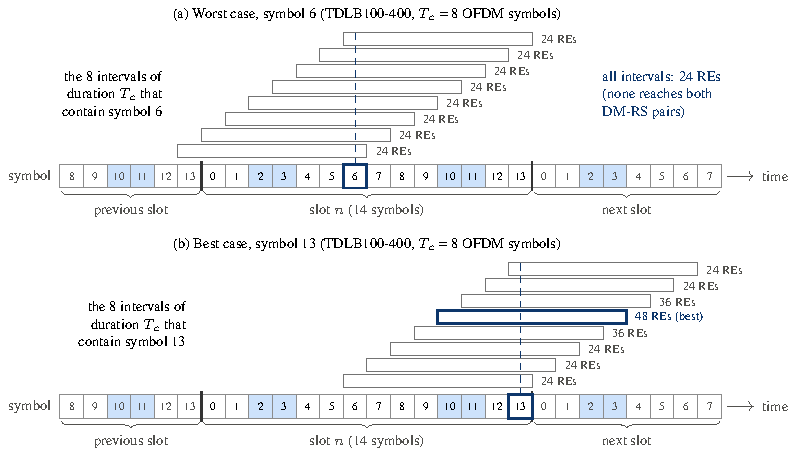
\includegraphics{Images/FLUXO/dmrs_n.pdf}
\vspace{4pt}
\legend{Source: the author, with the DM-RS positions of \citesp{3gpp-ts38211}. \textcolor{red}{Double-symbol DM-RS}, mapping type~A, symbols 2, 3, 10 and 11; continuous uplink. In (a) and (b), each bar is one position of an interval of duration $T_c$ that contains the marked symbol. Symbol 6 is the worst case of the slot, and symbol 13 is a best case.}
\end{figure}
